\documentclass{beamer}

\mode<presentation>{
\usetheme{Madrid}
%\usecolortheme{beaver}
}
\usepackage[utf8]{inputenc}
\usepackage{hyperref}
\usepackage{wrapfig}
\usepackage{graphicx}

\title[Big Data Analytics]{Big Data Analytics: Powering Systematic Strategies}
\author[CHEN Kai,HU Haoyu,ZHU Keyu]{CHEN Kai (12311410), HU Haoyu (12311225), ZHU Keyu (12313329)}
\institute[SUSTech]{Southern University of Science and Technology}
\date{April 16, 2025}


\begin{document}


\begin{frame}
 \maketitle
\end{frame}



\begin{frame}
\frametitle{Outline}
 \tableofcontents
\end{frame}



\section{Introduction}
\begin{frame}
\frametitle{Introduction}
\begin{minipage}{\textwidth}
\begin{itemize}
\setlength{\itemsep}{10pt}
    \item <1-> {\LARGE Question:}
    {\large Amount of data we generate?}
    \item <2-> {\LARGE \textbf{402.74 quintillion bytes/day}} (Duarte, 2025)
\end{itemize}
\begin{figure}
    \centering
    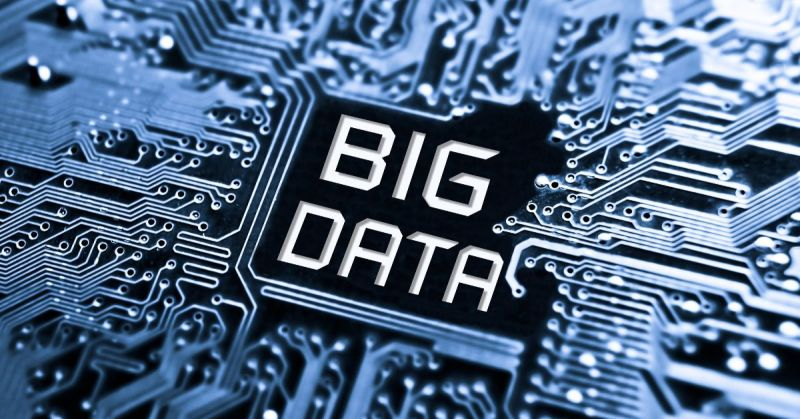
\includegraphics[width=0.5\linewidth]{figure 1.png}
    \label{fig:enter-label}
\end{figure}
\end{minipage}
\end{frame} 


\begin{frame}
 \frametitle{Introduction}
\begin{minipage}{\textwidth}
{\linespread{2}
\begin{itemize}
\item <1-> {\LARGE Big data enables systematic strategies}
    \begin{itemize}
        \item {\Large e.g. Data Mining, Machine Learning}
    \end{itemize}
\item <2-> {\LARGE Humans CANNOT manually analyze terabytes}
    \begin{itemize}
        \item {\Large Unstructured/ Massive data} (Ren, 2022)
    \end{itemize}
\end{itemize}
}
\end{minipage}
\end{frame}


\begin{frame}
 \frametitle{Introduction}
\begin{minipage}{\textwidth}
{\linespread{2}
\begin{itemize}
    \item {\LARGE Big data offers additional benefits:}
    \begin{itemize}
        \item <1-> {\large Uncover previously unnoticed patterns}
        \item <2-> {\large Powers personalized recommendation systems}
    \end{itemize}
\end{itemize}
}
\end{minipage}
\end{frame}



\section{Main Point 1: Discover Hidden Correlations}
\begin{frame}
 \frametitle{Main Point 1: Discover Hidden Correlations}
\begin{minipage}{\textwidth}
{\linespread{1.3}
\begin{itemize}
    \item {\Large Starting from a belief}
    \begin{itemize}
        \item {\large We Believe:}
        \item {\large EVERYTHING in the world}
        \item {\large Follows a “RULE” --- "ITS RULE"}
    \end{itemize}
\end{itemize}
}
\begin{figure}
    \centering
    \includegraphics[width=0.6\linewidth]{figure 8.png}
    \label{fig:enter-label}
\end{figure}
\end{minipage}
\end{frame}




\begin{frame}
 \frametitle{Main Point 1: Discover Hidden Correlations}
\begin{minipage}{\textwidth}
{\linespread{1.5}
\begin{itemize}
    \item <1-> {\Large Traditional Methods:}
    \begin{itemize}
        \item {\large Fail to identify some correlations}
        \item {\large e.g. supplier delays $\leftrightarrow$ production bottlenecks} (Ren, 2022)
    \end{itemize}
    \item <2-> {\Large Machine learning identifies non-obvious relationships}
    \begin{itemize}
        \item {\large e.g. weather patterns influencing logistics delays} (Ren, 2022)
    \end{itemize}
\end{itemize}
}
\begin{figure}
    \centering
    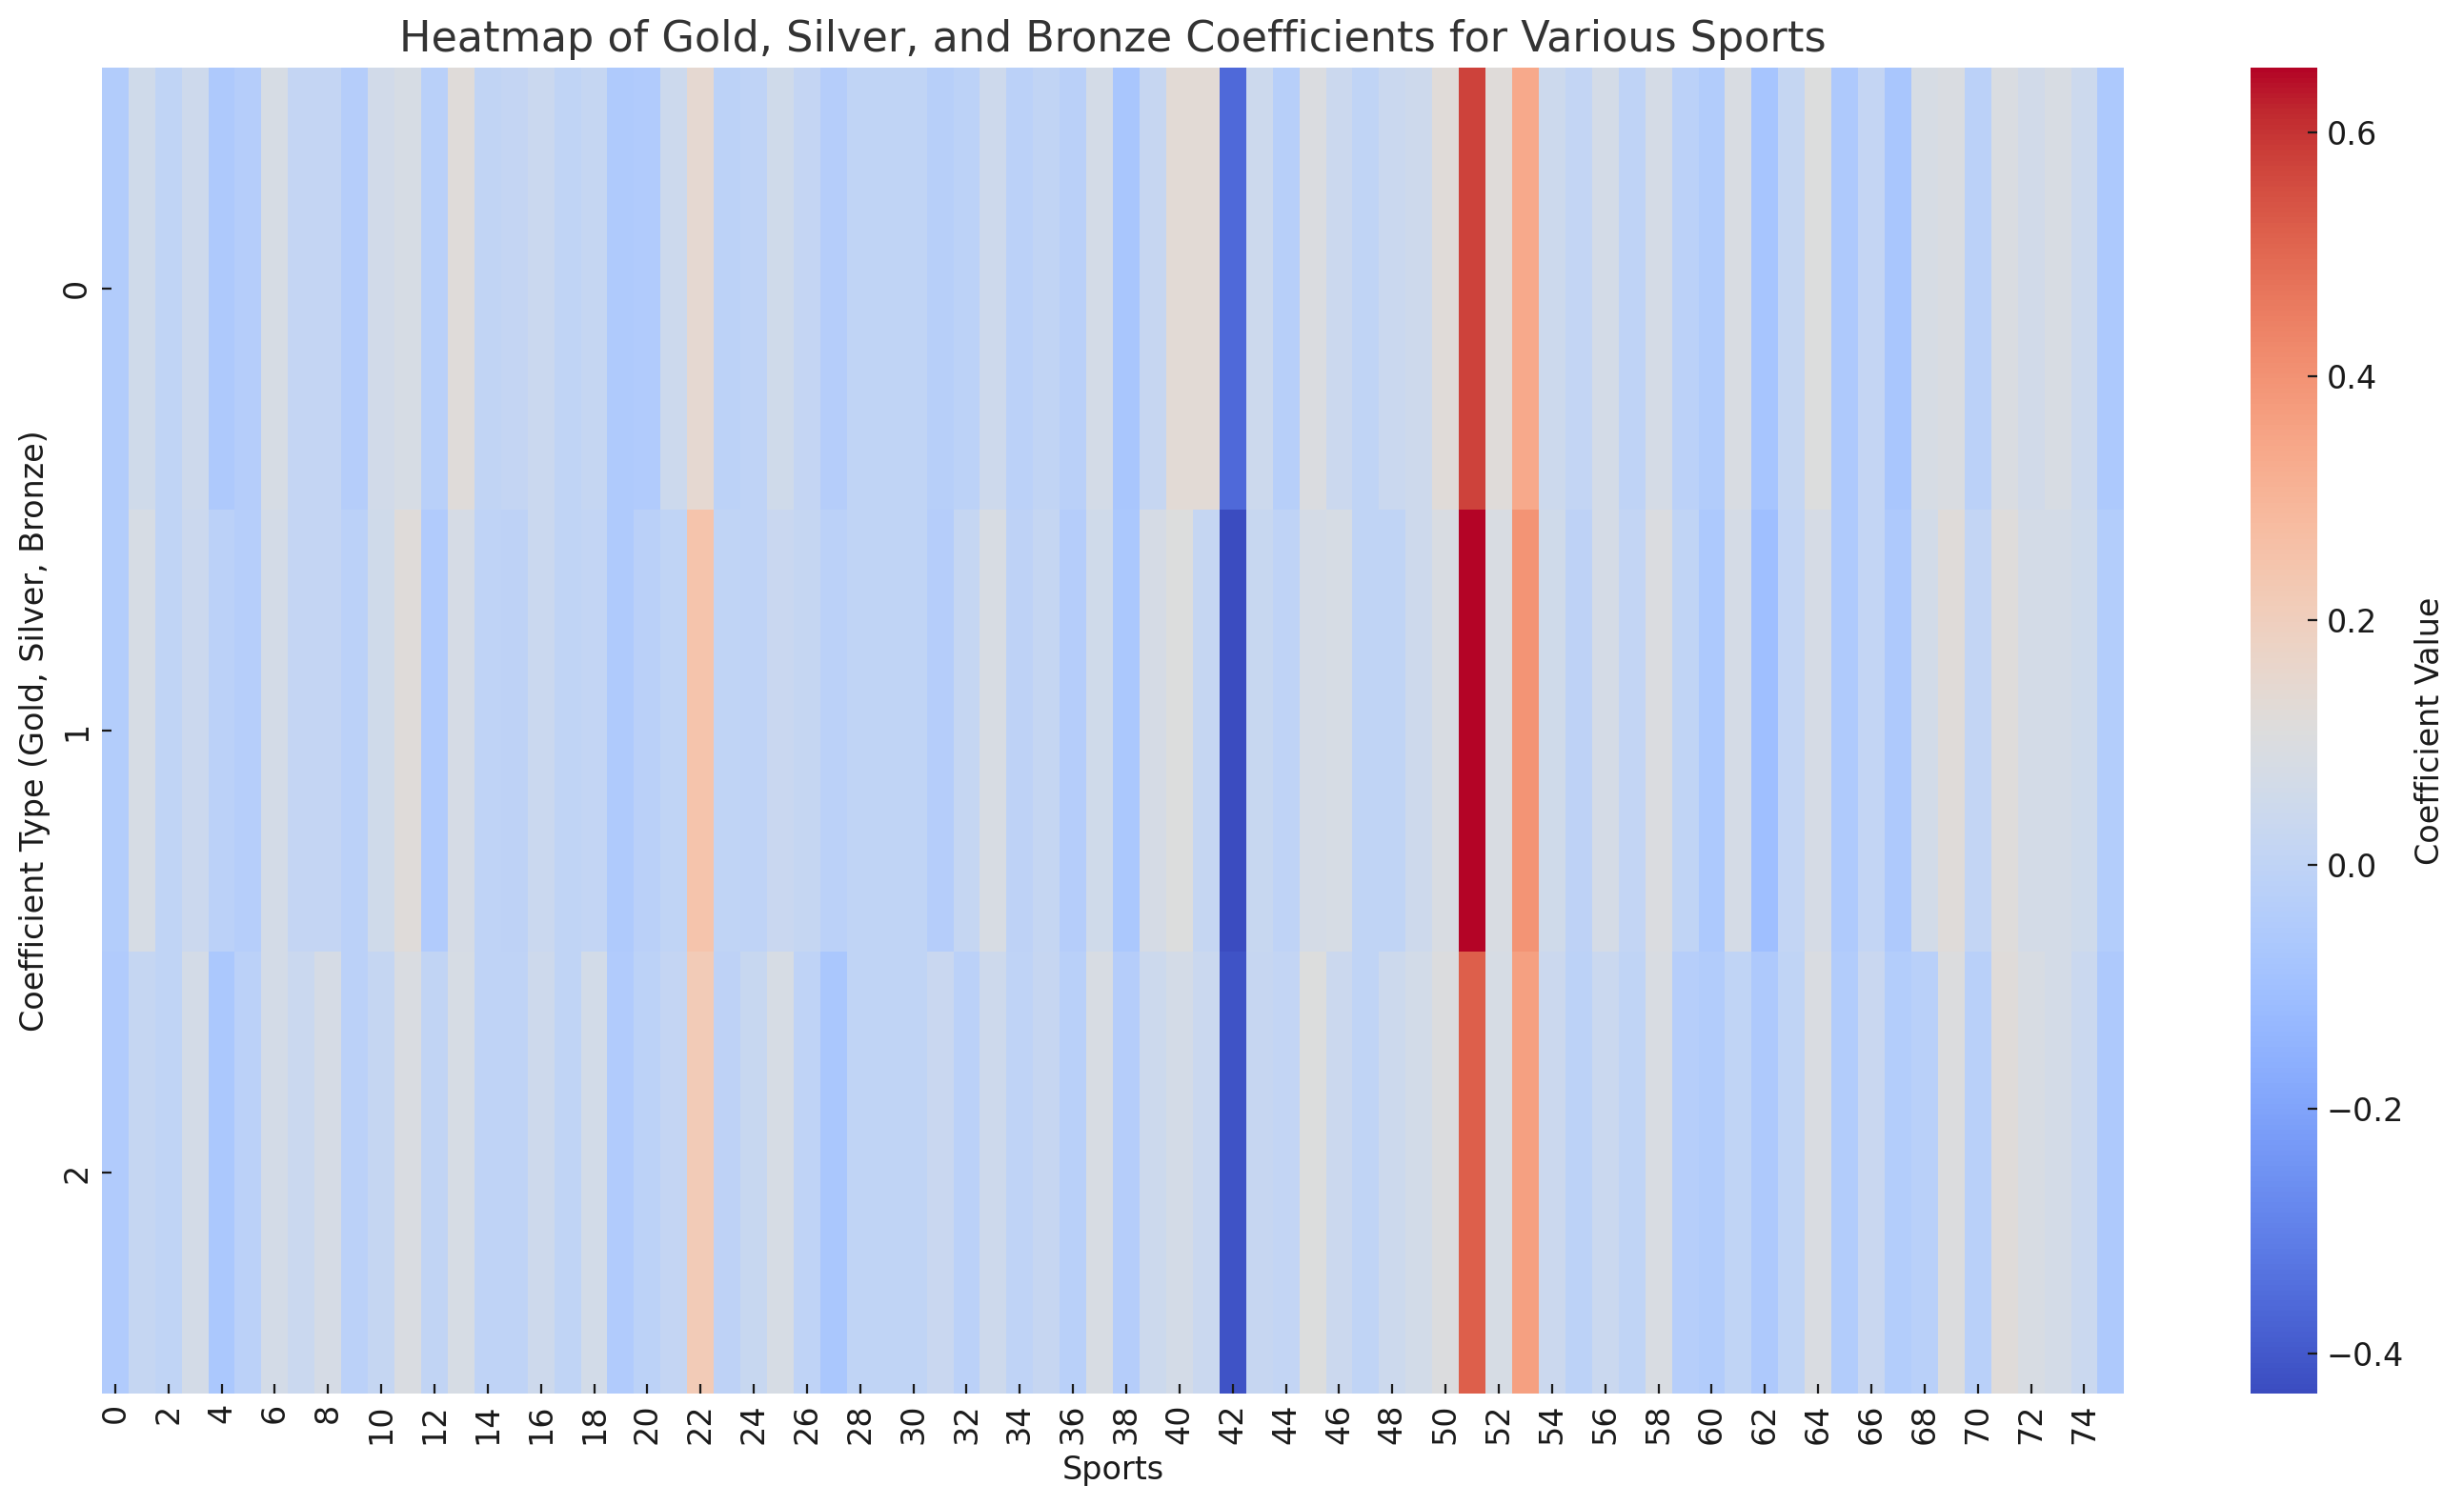
\includegraphics[width=0.5\linewidth]{Heatmap.png}
    \label{fig:enter-label}
\end{figure}
\end{minipage}
\end{frame}



\begin{frame}[t]
\frametitle{Main Point 1: Discover Hidden Correlations}
\begin{minipage}{\textwidth}
{\linespread{1.3}
\begin{itemize}
    \item {\Large A Case of My Own}
    \begin{itemize}
        \item {\large My experience in ACM}
        \item {\large case: anticipating Olympics medal tables}
    \end{itemize}
\end{itemize}
}

\vspace{0.7em} % 稍微缩小垂直间距

\centering
\tiny
\begin{tabular}{|c|c|c|c|c|c|c|c|c|c|c|c|c|}
\hline
\textbf{NOC} & \textbf{Golds} & \textbf{Gold\_low} & \textbf{Gold\_up} & \textbf{Silvers} & \textbf{Silver\_low} & \textbf{Silver\_up} & \textbf{Bronzes} & \textbf{Bronze\_low} & \textbf{Bronze\_up} & \textbf{Medals} & \textbf{Medals\_low} & \textbf{Medals\_up} \\
\hline
        USA & 49 & 38 & 59 & 37 & 27 & 45 & 35 & 25 & 40 & 121 & 90 & 144 \\
        CHN & 35 & 21 & 43 & 25 & 10 & 33 & 24 & 12 & 33 & 84 & 43 & 109 \\
        GBR & 21 & 14 & 30 & 18 & 8 & 26 & 19 & 11 & 26 & 58 & 33 & 82 \\
        GER & 13 & 2 & 21 & 14 & 8 & 23 & 21 & 15 & 28 & 48 & 25 & 72 \\
        FRA & 15 & 11 & 19 & 14 & 9 & 18 & 18 & 13 & 23 & 47 & 33 & 60 \\
        AUS & 14 & 7 & 20 & 12 & 6 & 18 & 18 & 13 & 22 & 44 & 26 & 60 \\
        JPN & 15 & 9 & 20 & 12 & 6 & 16 & 16 & 12 & 20 & 43 & 27 & 56 \\
        ITA & 12 & 10 & 16 & 12 & 10 & 15 & 14 & 12 & 17 & 38 & 32 & 48 \\
        CAN & 8 & 4 & 13 & 10 & 6 & 14 & 12 & 8 & 15 & 30 & 18 & 42 \\
        NED & 9 & 6 & 13 & 9 & 7 & 14 & 11 & 7 & 14 & 29 & 20 & 41 \\
        KOR & 9 & 0 & 14 & 7 & 0 & 12 & 6 & 0 & 12 & 22 & 0 & 36 \\
        ESP & 4 & 0 & 8 & 8 & 4 & 12 & 9 & 6 & 15 & 21 & 10 & 35 \\
        HUN & 7 & 5 & 11 & 6 & 4 & 9 & 7 & 4 & 10 & 20 & 13 & 30 \\
        BRA & 4 & 0 & 8 & 6 & 2 & 10 & 8 & 4 & 11 & 18 & 6 & 29 \\
        POL & 5 & 2 & 8 & 5 & 2 & 8 & 7 & 4 & 10 & 17 & 8 & 26 \\
        NZL & 6 & 4 & 9 & 5 & 2 & 7 & 6 & 3 & 8 & 17 & 9 & 24 \\
        UKR & 3 & 0 & 9 & 3 & 0 & 7 & 8 & 1 & 13 & 14 & 1 & 29 \\
        SWE & 3 & 1 & 6 & 5 & 1 & 7 & 5 & 3 & 8 & 13 & 5 & 21 \\
        CUB & 4 & 0 & 7 & 3 & 2 & 6 & 5 & 2 & 8 & 12 & 2 & 22 \\
\hline
\end{tabular}
\label{tab:medal_anticipation}
\end{minipage}
\end{frame}


\section{Main Point 2: Powering Personalized Recommendation}
\begin{frame}
 \frametitle{Main Point 2: Powering Personalized Recommendation}
\begin{minipage}{\textwidth}
{\linespread{1.3}
\begin{itemize}
    \item {\Large Precision Marketing in E-Commerce}
    \begin{itemize}
        \item <1-> {\large Analyze browsing/purchase data}
        \item <2-> {\large Dynamic user segmentation}
        \item <3-> {\large Case: 78.8\% conversion boost} (Luo, 2024)
    \end{itemize}
\end{itemize}
}
\begin{figure}
    \centering
    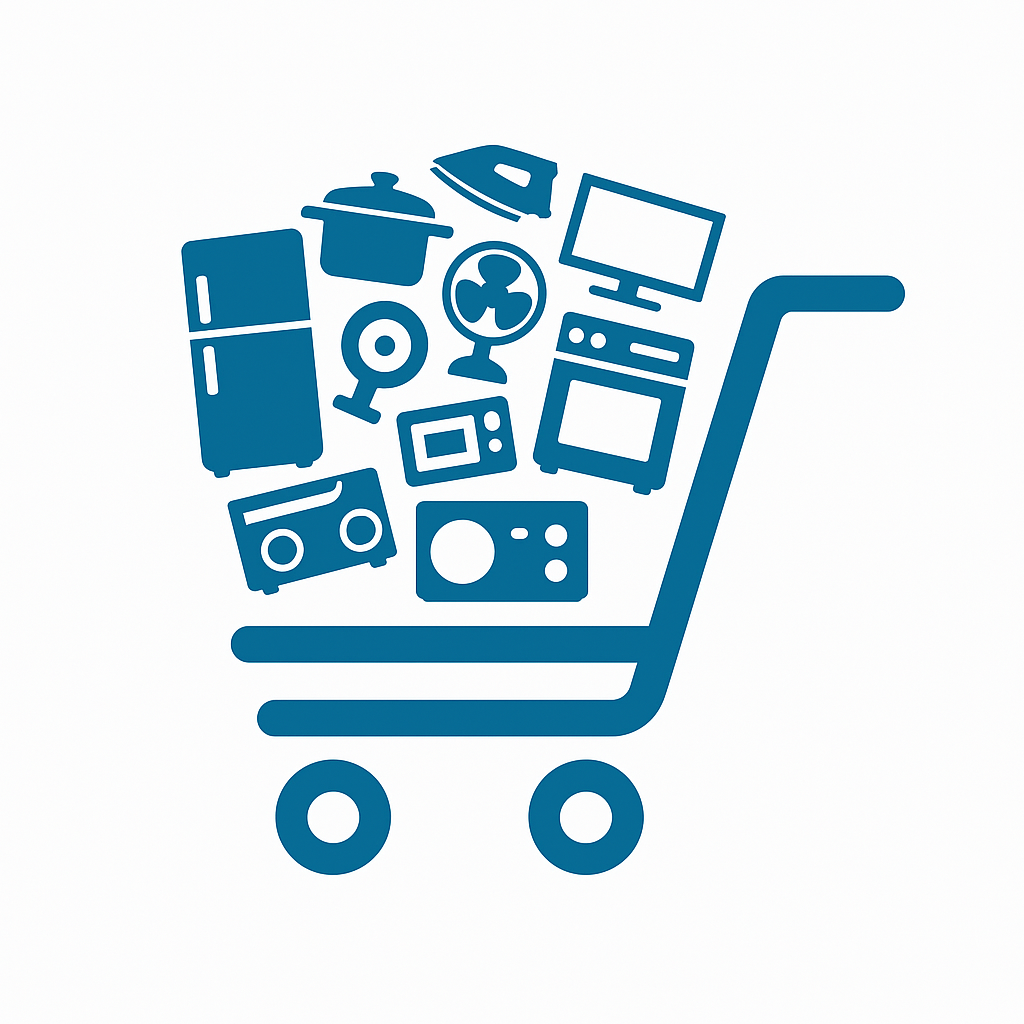
\includegraphics[width=0.35\linewidth]{figure 9.png}
    \label{fig:enter-label}
\end{figure}
\end{minipage}
\end{frame}



\begin{frame}
 \frametitle{Main Point 2: Powering Personalized Recommendation}
\begin{minipage}{\textwidth}
{\linespread{1.3}
\begin{itemize}
    \item {\Large Customized Solutions Across Industries}
    \begin{itemize}
        \item <1-> {\large Education: Adaptive learning} (Thimmanna et al., 2024)
        \item <2-> {\large Healthcare: Gene-based care} (Estape et al., 2016)
    \end{itemize}
\end{itemize}
}
\begin{figure}
    \centering
    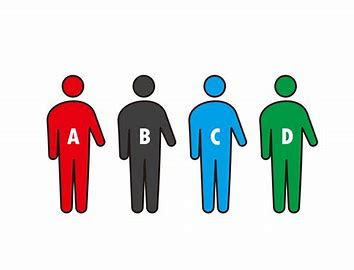
\includegraphics[width=0.45\linewidth]{figure 5.png}
    \label{fig:enter-label}
\end{figure}
\end{minipage}
\end{frame}



\section{Counterargument 1: Privacy Risk?}
\begin{frame}
 \frametitle{Counterargument 1: Privacy Risk?}
\begin{minipage}{\textwidth}
{\linespread{1.8}
\begin{itemize}
    \item <1-> {\Large Revealing sensitive user information}\\
    \begin{itemize}
        \item {\large e.g. Model Inversion Attacks} (Fredrikson et al. 2013)
    \end{itemize}
    \item <2-> {\Large However, mature technologies has emerged}
    \begin{itemize}
        \item {\large Function Secret Sharing (FSS)} (Ryffel et al., 2022)
        \item {\large Differential Privacy (DP) frameworks} (Das \& Mishra, 2024)
    \end{itemize}
    \item <3-> {\Large We have a mature toolkit!}
\end{itemize}
}

\end{minipage}
\end{frame}



\section{Counterargument 2: Tech Barrier?}
\begin{frame}
 \frametitle{Counterargument 2: Tech Barrier?}
\begin{minipage}{\textwidth}
{\linespread{1.8}
\begin{itemize}
    \item {\Large Algorithmic Complexity}\\
    \begin{itemize}
        \item <1-> {\large IMPA algorithm complexity}
        \item <2-> {\large High-dimension IoT delays}
        \item <3-> {\large Time-sensitive decision risks}
    \end{itemize}
    (Alrayes et al., 2025)
\end{itemize}
}

\end{minipage}
\end{frame}


\begin{frame}
 \frametitle{Counterargument 2: Tech Barrier?}
\begin{minipage}{\textwidth}
{\linespread{1.8}
\begin{itemize}
    \item {\Large Prohibitive Deployment Costs}
    \begin{itemize}
        \item <1-> {\large PPSLOA-HDBDE demands GPUs}
        \item <2-> {\large Edge deployment cost ×3-5}
        \item <3-> {\large Energy consumption alerts} 
    \end{itemize}
    (Alrayes et al., 2025)
\end{itemize}
}
\begin{figure}
    \centering
    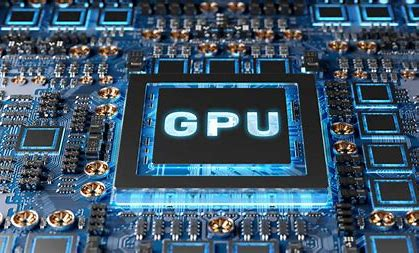
\includegraphics[width=0.35\linewidth]{figure 6.png}
    \label{fig:enter-label}
\end{figure}

\end{minipage}
\end{frame}


\section{Conclusion}
\begin{frame}
  \frametitle{Conclusion}

  \begin{wrapfigure}{r}{0.3\textwidth}
    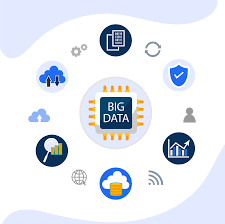
\includegraphics[width=0.28\textwidth]{figure 2.png}
    \label{fig:bigdata_conclusion}
  \end{wrapfigure}

  {\Large Big Data Analytics:}
  
  \vspace{2 em}
  
  {\Large \textbf{·} Uncovering hidden insights}
  
  \vspace{1 em}
  
  {\Large \textbf{·} Enabling intelligent personalization}
  
  \vspace{1.75 em}
  
  {\Large \textbf{·} Indispensable in modern society}

\end{frame}


\begin{frame}
 \frametitle{Conclusion}
\begin{minipage}{\textwidth}
{\Large \textbf{·} Data-driven personalized life enhancement}\\
\\{\Large \textbf{·} Big data analytics is everywhere}\\
\\
\\{\Large \textbf{·} Big data's expanding societal role}
\begin{figure}
    \centering
    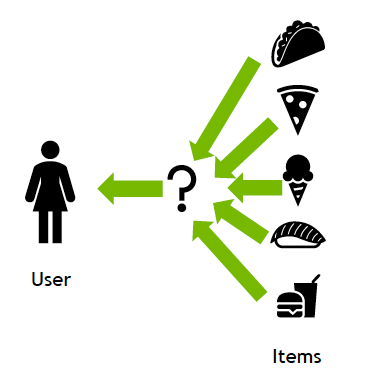
\includegraphics[width=0.35\linewidth]{figure 3.png}
    \label{fig:enter-label}
\end{figure}
\end{minipage}
\end{frame}



\section{References}
\begin{frame}
\frametitle{References}

\footnotesize
\begin{thebibliography}{5}

\bibitem{alrayes2025} Alrayes, F. S., Maray, M., Alshuhail, A., Almustafa, K. M., Darem, A. A., Al-Sharafi, A. M., \& Alotaibi, S. D. (2025). Privacy-preserving approach for IoT networks using statistical learning with optimization algorithm on high-dimensional big data environment. \emph{Scientific Reports}, \emph{15}(1). \href{https://doi.org/10.1038/s41598-025-87454-1}{https://doi.org/10.1038/s41598-025-87454-1}

\bibitem{das2024} Das, S., \& Mishra, S. (2024). Advances in Differential Privacy and Differentially Private Machine Learning [Preprint]. arXiv. \href{https://doi.org/10.48550/arXiv.2404.04706}{https://doi.org/10.48550/arXiv.2404.04706}

\bibitem{duarte2025} Duarte, F. (2025, March 28). Amount of data created daily (2025). \emph{Exploding Topics}. \href{https://explodingtopics.com/blog/data-generated-per-day}{https://explodingtopics.com/blog/data-generated-per-day}

\bibitem{estape2016} Estape, E. A., Mays, M. H., \& Sternke, E. A. (2016). Translation in Data Mining to Advance Personalized Medicine for Health Equity. \emph{Intelligent Information Management}, \emph{8}(1), 9-16. \href{https://doi.org/10.4236/iim.2016.81002}{https://doi.org/10.4236/iim.2016.81002}

\bibitem{fredrikson2015} Fredrikson, M., Jha, S., \& Ristenpart, T. (2015). Model inversion attacks that exploit confidence information and basic countermeasures. In \emph{Proceedings of the 22nd ACM SIGSAC Conference on Computer and Communications Security} (pp. 1322–1333). \href{https://doi.org/10.1145/2810103.2813677}{https://doi.org/10.1145/2810103.2813677}

\end{thebibliography}
\normalsize
\end{frame}



\begin{frame}
\frametitle{References}

\footnotesize
\begin{thebibliography}{5}

\bibitem{luo2024} Luo, Y. (2024). Optimization of product marketing and management path of cross-border e-commerce enterprises relying on big data technology. \emph{Applied Mathematics and Nonlinear Sciences}, \emph{9}(1), 1-19. \href{https://doi.org/10.2478/amns.2024.1.00001}{https://doi.org/10.2478/amns.2024.1.00001}

\bibitem{ren2022} Ren, S. (2022). Optimization of Enterprise Financial Management and Decision-Making Systems Based on Big Data. \emph{Journal of Mathematics}, \emph{2022}. \href{https://doi.org/10.1155/2022/1708506}{https://doi.org/10.1155/2022/1708506}

\bibitem{ryffel2022} Ryffel, T., Tholoniat, P., Pointcheval, D., \& Bach, F. (2022). AriaNN: Low-Interaction Privacy-Preserving Deep Learning via Function Secret Sharing. \emph{Proceedings on Privacy Enhancing Technologies}, \emph{2022}(1), 291–316. \href{https://doi.org/10.2478/popets-2022-0016}{https://doi.org/10.2478/popets-2022-0016}

\bibitem{thimmanna2024} Thimmanna, Sharma, A. V. N. S., Naik, M. S., Radhakrishnan, S., \& Sharma, A. (2024). Personalized Learning Paths: Adapting Education with AI-Driven Curriculum. \emph{European Economic Letters}, \emph{14}(1). \href{https://doi.org/10.52783/eel.v14i1.993}{https://doi.org/10.52783/eel.v14i1.993}

\end{thebibliography}
\normalsize
\end{frame}



\begin{frame}
\frametitle{Question and Answer}
{\Large Thank you for listening. Please feel free to ask questions!}
\end{frame}

\end{document}
